\section{Propuesta de Solución}

La propuesta presentada consiste en un sistema interactivo orientado a entornos ágiles, que permite optimizar la asignación de tareas dentro de un equipo de desarrollo mediante el uso de un algoritmo genético multiobjetivo. La solución busca balancear la carga de trabajo, minimizar el tiempo total de ejecución y considerar factores clave como dependencias, habilidades requeridas y costos asociados.

El sistema se estructura en torno a una arquitectura modular que separa claramente la interfaz de usuario, la lógica de negocio y el motor de optimización. Esta separación permite una interacción clara y eficiente con el usuario, al mismo tiempo que encapsula la complejidad de la heurística evolutiva implementada.

En las siguientes subsecciones se detalla el modelo general del sistema, el diseño del algoritmo genético propuesto, y la forma en que los componentes se integran para generar una solución viable y extensible al problema de asignación de tareas.

\subsection{Modelo General del Sistema}

Como se representó anteriormente en la Figura~\ref{fig:arquitectura}, el sistema está compuesto por tres componentes principales: \textbf{Interfaz Gráfica}, \textbf{API} y \textbf{Núcleo de Optimización}.

\begin{itemize}
    \item \textbf{Interfaz Gráfica}: Permite al usuario visualizar los resultados y configurar parámetros clave del algoritmo genético, como el tamaño de la población, número de generaciones, tasas de cruce y mutación, tamaño del torneo y los pesos de la función objetivo.

    \item \textbf{API}: Recibe las configuraciones del usuario y los datos estáticos de tareas y desarrolladores. Actúa como intermediario entre la interfaz gráfica y el núcleo del algoritmo, enviando y recibiendo información a través de endpoints definidos en Flask.

    \item \textbf{Núcleo de Optimización}: Implementado en Python, este módulo contiene la lógica completa del algoritmo genético. Se encarga de generar soluciones viables y optimizadas para la asignación de tareas, respetando restricciones de dependencias, habilidades, tiempos y costos.
\end{itemize}

Esta aproximación cliente-servidor con separación clara entre capas permite al usuario interactuar de forma sencilla con la aplicación, facilitando la configuración de parámetros y la visualización de resultados, todo mientras se mantiene encapsulada la complejidad interna del algoritmo genético multiobjetivo para la optimización de la asignación de tareas.

\subsection{Algoritmo Genético Propuesto}

El núcleo del sistema implementa un \textbf{algoritmo genético multiobjetivo} para resolver el problema de asignación de tareas bajo múltiples restricciones prácticas. Esta técnica de optimización evolutiva busca simultáneamente minimizar o balancear varios factores conflictivos mediante una \textit{función de evaluación compuesta}, lo cual distingue este enfoque de soluciones más simples o unidimensionales.

Como ya fue ilustrado en la Figura~\ref{fig:flujo}, el algoritmo parte de una población aleatoria de asignaciones. A través de ciclos generacionales, se aplican los operadores clásicos de selección, cruce y mutación, buscando mejorar progresivamente la calidad de las soluciones candidatas.

\begin{itemize}
    \item \textbf{Función de evaluación compuesta (multiobjetivo):}  
La aptitud de cada cromosoma se determina mediante una combinación ponderada de múltiples criterios:

\begin{itemize}
    \item \textbf{Makespan:} duración total del sprint.
    \item \textbf{Balance de carga:} distribución equitativa del esfuerzo.
    \item \textbf{Habilidades:} ajuste entre habilidades requeridas y ofrecidas.
    \item \textbf{Costo estimado:} según tarifas por hora de cada desarrollador.
\end{itemize}

Los pesos asignados a cada uno de estos criterios pueden ser definidos por el usuario desde la interfaz del sistema. Este aspecto se detalla más adelante en la Sección~\ref{sec:evaluacion}.

    \item \textbf{Verificación previa y caché:} Se implementa una caché que almacena los valores de fitness ya evaluados para evitar recomputaciones innecesarias. Asimismo, las tareas se ordenan topológicamente antes del proceso evolutivo para asegurar que las dependencias entre ellas se respeten desde el inicio.

    \item \textbf{Operadores genéticos personalizados:}  
Se adaptaron los operadores clásicos del algoritmo genético para cumplir con las restricciones específicas del problema:

\begin{itemize}
    \item \textbf{Selección por torneo:} elección competitiva aleatoria.
    \item \textbf{Cruce por segmentos:} combina parcialmente asignaciones entre padres.
    \item \textbf{Mutación por reasignación:} cambio aleatorio de tarea.
    \item \textbf{Corrección posterior:} validación de soluciones generadas.
    \item \textbf{Elitismo parcial:} preserva el mejor individuo en cada generación.
\end{itemize}

Estos mecanismos se describen en detalle en la Sección~\ref{sec:operadores}.

    \item \textbf{Mecanismo de paciencia (estancamiento):} Si durante un número consecutivo de generaciones no se encuentra una mejor solución, el algoritmo se detiene anticipadamente, optimizando el tiempo de ejecución sin comprometer la calidad.
\end{itemize}

Este enfoque multiobjetivo permite una exploración equilibrada del espacio de soluciones, adaptándose a prioridades definidas por el usuario y garantizando asignaciones válidas, eficientes y costo-efectivas de las tareas disponibles.

% \subsection{Algoritmo Genético Propuesto}

% El núcleo de optimización sigue un enfoque evolutivo, donde una población inicial de soluciones (cromosomas) se somete a iteraciones de evaluación, selección, cruce y mutación para mejorar la asignación de tareas.

% \begin{itemize}
%     \item Se parte de una población aleatoria de asignaciones.
%     \item Cada generación aplica operadores genéticos y se evalúan las soluciones.
%     \item La mejor solución se toma como sprint generado.
%     \item El proceso se repite hasta vaciar el backlog.
% \end{itemize}

% \noindent\textbf{Imagen:} \textit{(opcional)} flujograma simple del algoritmo. Ej: pseudodiagrama basado en 'while tareas\_pendientes:'.

\subsection{Representación de Soluciones}

En el contexto del algoritmo genético propuesto, cada solución candidata —también llamada cromosoma— representa una asignación completa de tareas a desarrolladores para un sprint específico. Esta asignación se codifica como una lista ordenada de identificadores de desarrolladores, donde la posición de cada elemento corresponde a una tarea según un orden topológico que respeta las dependencias del proyecto.

\textbf{Ejemplo de representación:}
Supóngase un conjunto de cuatro tareas ordenadas como $[T_0, T_1, T_2, T_3]$ y un cromosoma dado por la secuencia $[2, 1, 1, 3]$. Esto implica que:
\begin{itemize}
    \item La tarea $T_0$ se asigna al desarrollador con ID 2.
    \item La tarea $T_1$ se asigna al desarrollador con ID 1.
    \item La tarea $T_2$ también se asigna al desarrollador 1.
    \item La tarea $T_3$ se asigna al desarrollador con ID 3.
\end{itemize}

Dado que no todas las tareas pueden resolverse en un solo sprint —debido a restricciones de tiempo o dependencias—, el algoritmo aplica esta lógica de forma iterativa. Es decir, genera una secuencia de cromosomas (uno por sprint) hasta que se completa la asignación de todas las tareas del backlog. Cada uno de estos cromosomas constituye una solución parcial, y el conjunto completo representa la solución total del sistema.

Una forma simple de visualizar esta asignación es mediante una tabla que agrupe las tareas por sprint, detallando a qué desarrollador se asignó cada una de ellas y los tiempos estimados de ejecución.

\begin{center}
    \begin{tabular}{|c|c|c|c|c|}
        \hline
        \textbf{Sprint} & \textbf{Tarea} & \textbf{Desarrollador} & \textbf{Inicio (h)} & \textbf{Fin (h)} \\
        \hline
        1               & T0             & Dev 2                  & 0                   & 3                \\
        1               & T1             & Dev 1                  & 0                   & 5                \\
        1               & T2             & Dev 1                  & 5                   & 10               \\
        1               & T3             & Dev 3                  & 0                   & 4                \\
        \hline
        2               & T4             & Dev 2                  & 0                   & 4                \\
        2               & T5             & Dev 1                  & 0                   & 3                \\
        2               & T6             & Dev 3                  & 0                   & 2                \\
        \hline
    \end{tabular}
\end{center}

De esta forma, podemos ver claramente tanto la estructura de un cromosoma individual —con sus tareas asignadas, desarrolladores responsables y tiempos estimados— como el conjunto completo de cromosomas que, distribuidos por sprint, conforman una solución integral.

Este conjunto final de cromosomas constituye la salida principal del algoritmo, y será posteriormente interpretado por la interfaz del usuario, que se encargará de presentarlo de forma comprensible y útil para el usuario final.

% \subsection{Representación de Soluciones}

% Cada cromosoma representa una posible asignación de tareas a desarrolladores. Esta representación codifica:

% \begin{itemize}
%     \item Qué tareas se asignan a qué programadores.
%     \item El orden en que deben completarse (respetando dependencias).
%     \item El ajuste según las habilidades de cada desarrollador.
% \end{itemize}

% \noindent\textbf{Imagen:} \textit{(opcional)} ejemplo visual de un cromosoma o tabla de asignaciones (opcional si ya lo describes en texto).

\subsection{Evaluación de Soluciones (Función Objetivo)}
\label{sec:evaluacion}

La calidad de cada solución candidata —representada por un cromosoma— es evaluada mediante una función objetivo compuesta que pondera múltiples criterios relevantes para la planificación ágil de proyectos. Esta función busca minimizar los siguientes aspectos:

\begin{itemize}
    \item \textbf{Makespan (50\%)}: tiempo total requerido para completar todas las tareas asignadas, considerando las dependencias y la disponibilidad de cada desarrollador.
    \item \textbf{Varianza de carga (25\%)}: medida de desequilibrio en la cantidad de trabajo distribuido entre desarrolladores. Cuanto menor sea, más balanceado es el plan.
    \item \textbf{Coincidencia de habilidades (20\%)}: penalización proporcional a la diferencia entre los niveles de habilidad requeridos por una tarea y los ofrecidos por el desarrollador asignado.
    \item \textbf{Costo total (5\%)}: estimado en función de las horas trabajadas por cada desarrollador y su tarifa horaria.
\end{itemize}

Todos estos valores son combinados mediante una fórmula ponderada de la siguiente forma:

\[
    \text{Fitness} = w_1 \cdot \text{Makespan} + w_2 \cdot \text{Varianza} + w_3 \cdot \text{SkillGap} + w_4 \cdot \text{Costo}
\]

Donde los pesos $(w_1, w_2, w_3, w_4)$ son definidos por el usuario a través de la interfaz del sistema y, por defecto, corresponden a $(0.5,\ 0.25,\ 0.2,\ 0.05)$.

Además, si una solución incumple restricciones críticas —como exceder la capacidad horaria de un desarrollador o asignar tareas con brechas de habilidad excesivas— se le asigna automáticamente una penalización severa definida como \texttt{BIG\_PENALTY}. Esto permite descartar de forma eficiente los cromosomas inviables sin necesidad de mantenerlos durante el proceso evolutivo.

\noindent\textbf{Pseudocódigo de evaluación:}

\begin{verbatim}
function evaluate_chromosome(chromosome):
    asignar tareas a desarrolladores según cromosoma
    calcular makespan total
    calcular varianza de carga entre desarrolladores
    calcular penalización por brechas de habilidades
    calcular costo total estimado

    if capacidad excedida o penalización muy alta:
        return BIG_PENALTY

    return w1*makespan + w2*varianza + w3*penalización + w4*costo
\end{verbatim}

Gracias a esta evaluación compuesta, el algoritmo puede priorizar soluciones más equilibradas y alineadas con los objetivos del sistema, al considerar simultáneamente múltiples criterios derivados de las restricciones del problema.

Esta función actúa como el eje central del proceso evolutivo, guiando la búsqueda hacia asignaciones óptimas dentro de un espacio de soluciones complejo y condicionado por las tareas y los perfiles de los desarrolladores disponibles.

% \subsection{Evaluación de Soluciones (Función Objetivo)}

% La función objetivo pondera múltiples criterios para determinar la calidad de una solución:

% \begin{itemize}
%     \item \textbf{Makespan (50\%)}: duración del sprint.
%     \item \textbf{Balance de carga (25\%)}: varianza en horas por developer.
%     \item \textbf{Coincidencia de habilidades (20\%)}: afinidad entre habilidades requeridas y ofrecidas.
%     \item \textbf{Costo (5\%)}: según tarifas por hora.
% \end{itemize}

% \noindent\textbf{Imagen:} \textit{(opcional)} fórmula matemática o pseudocódigo de evaluación.

\subsection{Operadores Genéticos Personalizados}
\label{sec:operadores}

Una vez evaluadas las soluciones candidatas mediante la función objetivo, el algoritmo debe decidir cuáles de ellas continuarán participando en el proceso evolutivo. Para ello, se emplean los operadores genéticos clásicos propios de esta familia de algoritmos, como la selección, el cruce y la mutación, que permiten generar nuevas combinaciones de asignaciones a partir de las existentes.

En nuestro contexto particular, dichos operadores fueron adaptados para respetar las restricciones del problema, evitando asignaciones inválidas y promoviendo la diversidad sin comprometer la validez de las soluciones. Esto dio lugar a un conjunto de operadores genéticos personalizados, cuya función es guiar de forma eficiente la exploración del espacio de soluciones, favoreciendo la mejora progresiva de la población en cada generación.

A continuación se detallan los operadores personalizados implementados en el sistema:

\begin{itemize}
\item \textbf{Selección por torneo:} Se elige aleatoriamente un subconjunto de soluciones candidatas y se selecciona la mejor entre ellas. Este método favorece un equilibrio entre explotación y diversidad, evitando la convergencia prematura a soluciones subóptimas.

\item \textbf{Cruce por segmentos:} A partir de dos soluciones padres, se toma un segmento de asignaciones de uno de ellos y se completa la solución con los valores del otro, cuidando no violar restricciones como dependencias o exceso de carga por desarrollador.

\item \textbf{Mutación por reasignación:} Con una baja probabilidad, se modifica la asignación de una tarea a otro desarrollador válido. Esta operación introduce variación genética y ayuda a explorar regiones no visitadas del espacio de búsqueda.

\item \textbf{Corrección postoperadores:} Tras aplicar cruce o mutación, se verifica que la solución resultante sea válida. Esto incluye evitar duplicaciones indebidas, respetar capacidades, y garantizar el cumplimiento de las dependencias entre tareas.

\item \textbf{Elitismo parcial:} En cada generación, se preserva el mejor cromosoma encontrado hasta el momento, garantizando que los avances evolutivos no se pierdan. Esta élite se mantiene limitada para no comprometer la diversidad genética de la población.
\end{itemize}

Gracias a estos operadores personalizados, el algoritmo puede generar soluciones viables incluso en escenarios altamente restringidos, manteniendo un equilibrio entre exploración y explotación durante todo el proceso evolutivo.

% \subsection{Operadores Genéticos Personalizados}

% Los operadores han sido ajustados para respetar restricciones del problema:

% \begin{itemize}
%     \item \textbf{Selección:} por torneo.
%     \item \textbf{Cruce:} combinación parcial de asignaciones entre padres.
%     \item \textbf{Mutación:} reasignación de tareas con baja probabilidad.
%     \item \textbf{Corrección:} validación para evitar duplicados y tareas inválidas.
% \end{itemize}

% \noindent\textbf{Imagen:} no requerida, puede ser solo texto.

\subsection{Interacción con la Interfaz Web}

El sistema incluye una interfaz web intuitiva que permite al usuario gestionar todo el flujo de trabajo: carga de datos, configuración del algoritmo, ejecución del proceso evolutivo y visualización de resultados optimizados.

\subsubsection{Visualización de Datos de Tareas y Desarrolladores}
La interfaz incluye secciones dedicadas para consultar las tareas y desarrolladores definidos en el sistema. Estas páginas permiten al usuario revisar propiedades clave como esfuerzo estimado, habilidades requeridas, prioridades, capacidades y costos por hora.

Si bien actualmente no se admite la carga dinámica de datos desde la interfaz, el sistema trabaja con un conjunto representativo de tareas y desarrolladores de prueba. Este conjunto es suficiente para validar el funcionamiento del algoritmo y visualizar sus resultados en un entorno controlado.

\begin{figure}[htbp]
    \centering
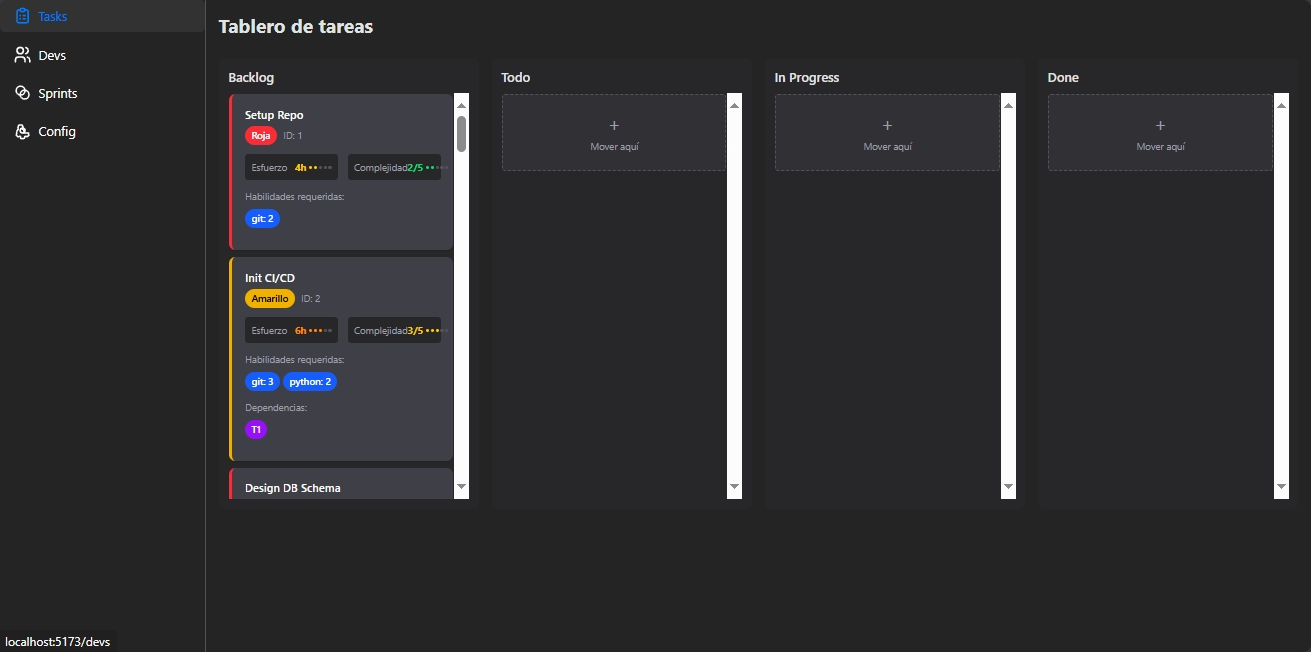
\includegraphics[width=0.9\textwidth]{imagenes/web-tasks.png}
    \caption{Pestaña de tablero de tareas disponibles.}
    \label{fig:tareas}
\end{figure}

\begin{figure}[htbp]
    \centering
    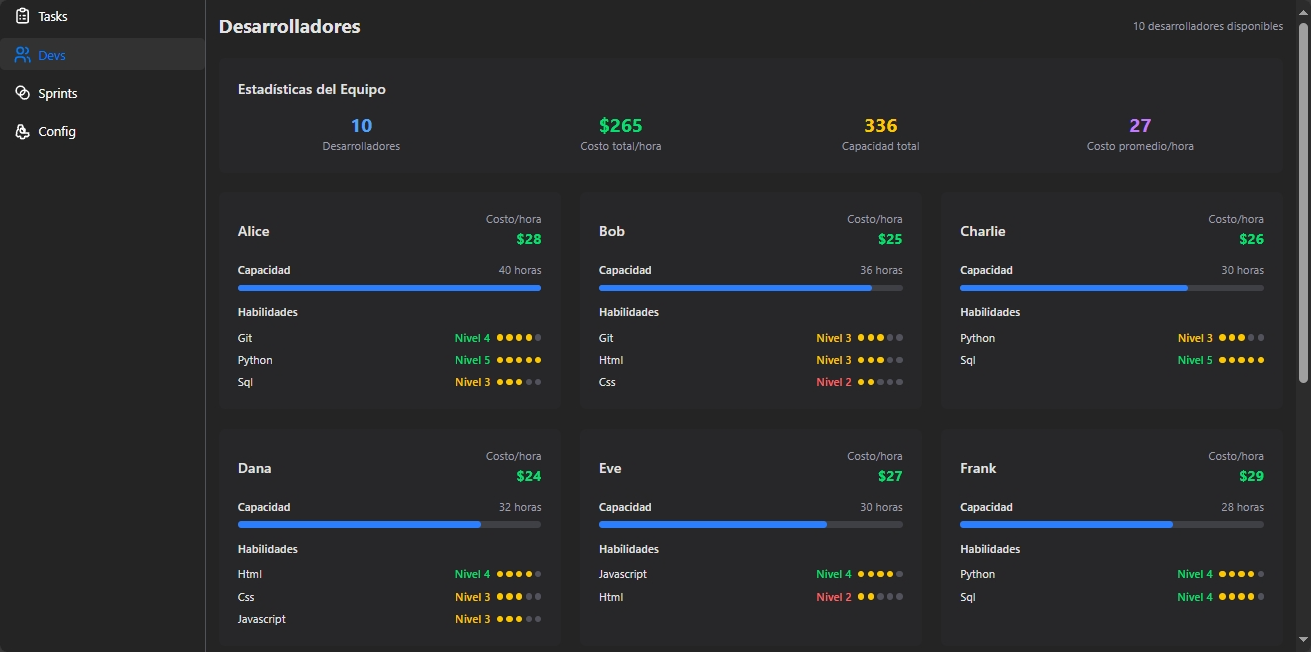
\includegraphics[width=0.9\textwidth]{imagenes/web-devs.png}
    \caption{Pestaña de desarrolladores definidos.}
    \label{fig:desarrolladores}
\end{figure}

\subsubsection{Configuración de Parámetros del Algoritmo}
La interfaz permite ajustar los parámetros clave que gobiernan el comportamiento del algoritmo genético. Estos incluyen el tamaño de la población, el número máximo de generaciones, las tasas de cruce y mutación, el tamaño del torneo de selección, y los pesos asignados a cada uno de los criterios de evaluación.

Esta configuración flexible permite experimentar con distintas estrategias evolutivas según las necesidades del usuario.

\begin{figure}[htbp]
    \centering
    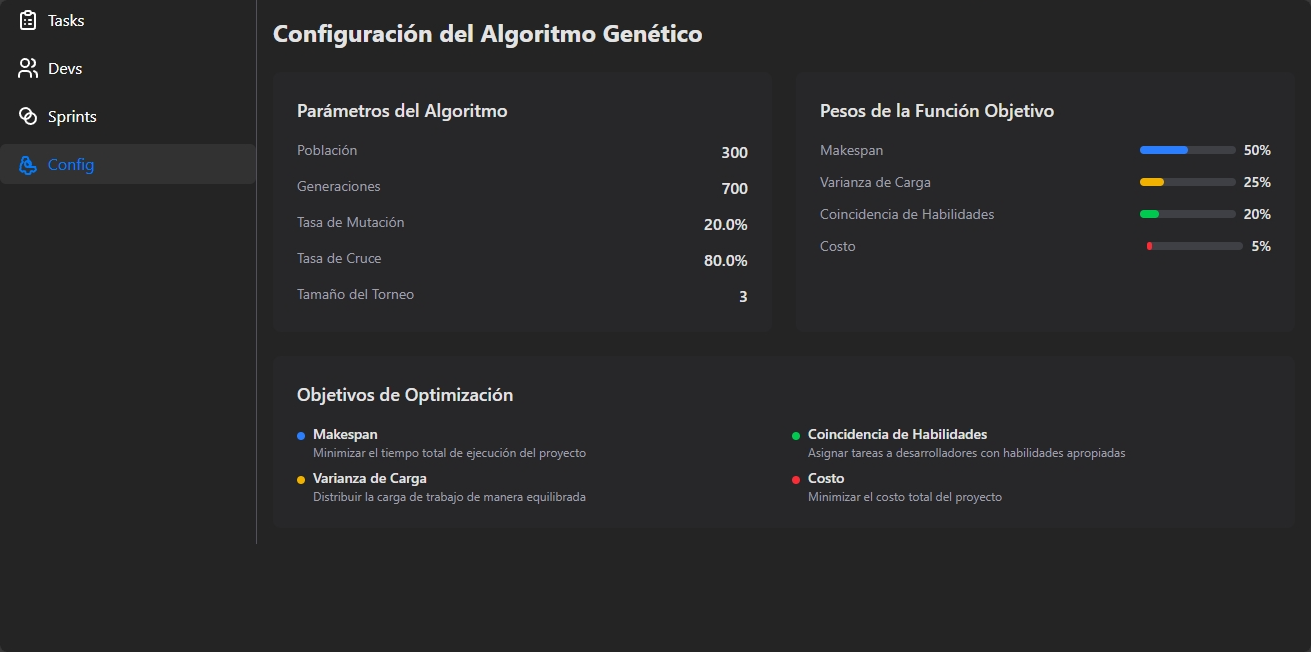
\includegraphics[width=0.9\textwidth]{imagenes/web-config.png}
    \caption{Panel de configuración del algoritmo genético.}
    \label{fig:config}
\end{figure}

\subsubsection{Ejecución del Algoritmo y Visualización de Resultados}
Una vez definidos los datos y parámetros, el usuario puede ejecutar el algoritmo desde la sección correspondiente. El sistema procesa las asignaciones y genera uno o varios sprints optimizados que se presentan visualmente.

Cada resultado muestra qué tareas fueron asignadas a cada desarrollador, la duración del sprint (makespan) y la prioridad de las tareas incluidas, permitiendo evaluar rápidamente la calidad de la solución generada.

\begin{figure}[htbp]
    \centering
    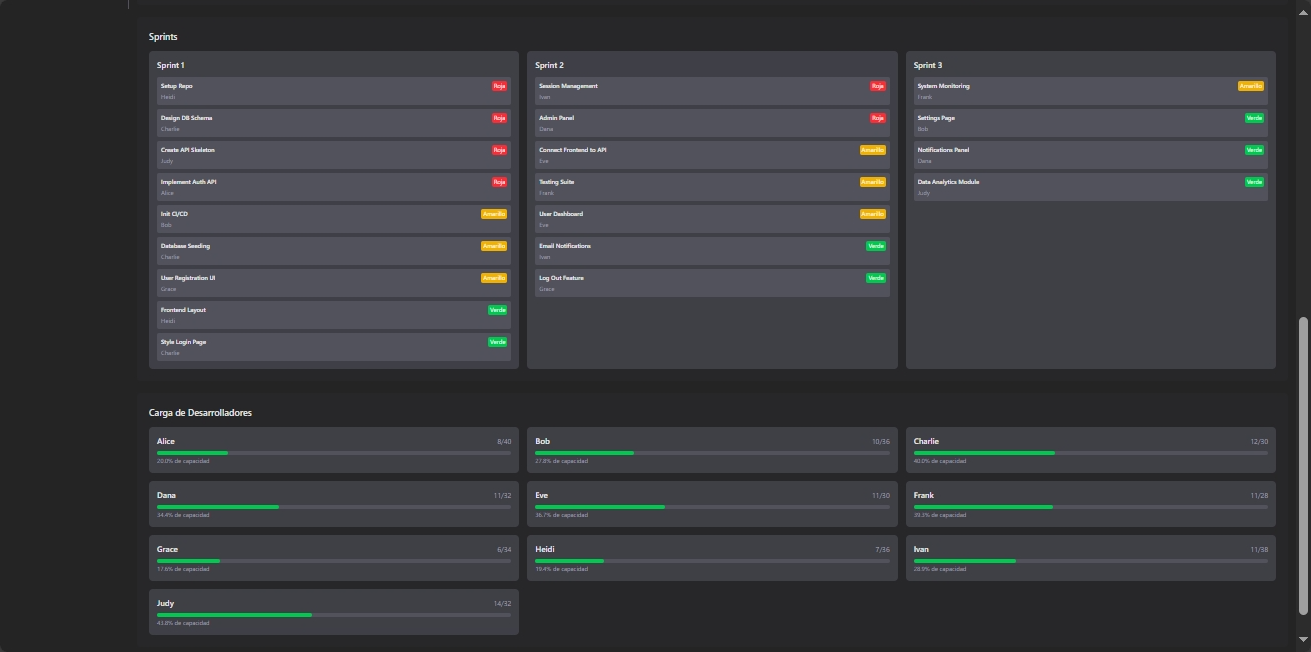
\includegraphics[width=0.9\textwidth]{imagenes/web-sprints.png}
    \caption{Visualización de los sprints generados por el algoritmo.}
    \label{fig:resultados}
\end{figure}

\subsubsection*{Cierre del Proceso}

Con esta secuencia completa —desde la visualización de los datos base, pasando por la configuración personalizada del algoritmo, hasta la ejecución del proceso evolutivo y la interpretación de sus resultados— se cubre todo el ciclo de uso del sistema propuesto.

Este flujo integral permite al usuario obtener soluciones optimizadas de forma accesible y comprensible, facilitando así la toma de decisiones informadas dentro de contextos reales de planificación y asignación de tareas.

% \subsection{Interfaz y Configuración del Usuario}

% El sistema permite que el usuario ajuste los parámetros del algoritmo genético desde una interfaz web amigable:

% \begin{itemize}
%     \item Población inicial
%     \item Número de generaciones
%     \item Tasa de mutación y cruce
%     \item Tamaño del torneo
%     \item Pesos para cada criterio de evaluación
% \end{itemize}

% \noindent\textbf{Imagen:} captura del frontend (panel de configuración).

% \subsection{Ejemplo de Ejecución}

% Se realizó una ejecución completa con el conjunto estático de tareas y desarrolladores. Se configuraron los parámetros del algoritmo y se generaron varios sprints:

% \begin{itemize}
%     \item Se obtuvo un conjunto de sprints con carga balanceada.
%     \item Las tareas respetaron todas sus dependencias.
%     \item El makespan fue razonable para el conjunto dado.
% \end{itemize}

% \noindent\textbf{Imagen:} \textit{opcional} captura de los resultados visualizados (por ejemplo, tabla con desarrolladores y tareas).


% La propuesta consiste en un sistema capaz de asignar automáticamente tareas a desarrolladores en base a un modelo evolutivo. El sistema considera el esfuerzo estimado por tarea, las dependencias entre ellas y la disponibilidad de los miembros del equipo.

% El algoritmo genético es ajustado para minimizar el desequilibrio de carga, respetar las restricciones impuestas por los sprints y optimizar el flujo de trabajo. La solución incluye un módulo de visualización que muestra la distribución sugerida.

% \vspace{0.5cm}

% \begin{tcolorbox}[colback=gray!10, colframe=black!30, title={Sugerencias para esta sección}]
%     \begin{itemize}
%         \item Explica brevemente qué hace tu solución y cómo se integra en un entorno ágil.
%         \item Muestra capturas o diagramas si ya has hecho avances de código.
%         \item Puedes separar en módulos: asignación, evaluación, visualización.
%         \item Justifica por qué tu propuesta mejora lo que ya existe.
%     \end{itemize}
% \end{tcolorbox}